\documentclass[12pt]{article}

\usepackage{subcaption}
\usepackage{float}
\usepackage{graphicx}
\usepackage{listings}
\usepackage[hidelinks]{hyperref}
\usepackage[super]{nth}
\graphicspath{{data/}}

\usepackage{xcolor}

\definecolor{codegreen}{rgb}{0,0.6,0}
\definecolor{codegray}{rgb}{0.5,0.5,0.5}
\definecolor{codepurple}{rgb}{0.58,0,0.82}
\definecolor{backcolour}{rgb}{0.95,0.95,0.92}

\lstdefinestyle{mystyle}{
backgroundcolor=\color{backcolour},
commentstyle=\color{codegreen},
keywordstyle=\color{magenta},
numberstyle=\tiny\color{codegray},
stringstyle=\color{codepurple},
basicstyle=\ttfamily\footnotesize,
breakatwhitespace=false,
breaklines=true,
captionpos=b,
keepspaces=true,
numbers=left,
numbersep=5pt,
showspaces=false,
showstringspaces=false,
showtabs=false,
tabsize=2
}

\lstset{style=mystyle}

\textheight 23.2 cm

\textwidth 6.0 in

\hoffset = -0.5 in

\voffset = -2.4 cm

\hyphenation{}

\frenchspacing

\title{
\large Introduction to image processing and computer vision \\
\LARGE \textbf{Plant Species Recognition} \\
Laboratory Project 2
}

\author{Patryk Walczak}

\begin{document}

\maketitle

\tableofcontents

\thispagestyle{empty}

\newpage

\clearpage
\pagenumbering{arabic}

\section{Introduction}

\paragraph{
The main task of the project is an elaboration of a discriminative feature vector for the leaves of trees. Using computer vision processing find the vectors then learn the machine learning model with 80\% of the data set and test the results on the remaining part. Six tree species each in the separated dictionary are stored in "isolated" dictionary. In each class is from 38 up to 97 images of leaves.
}


\begin{figure}[b!]
\centering
\begin{subfigure}[b]{0.3\textwidth}
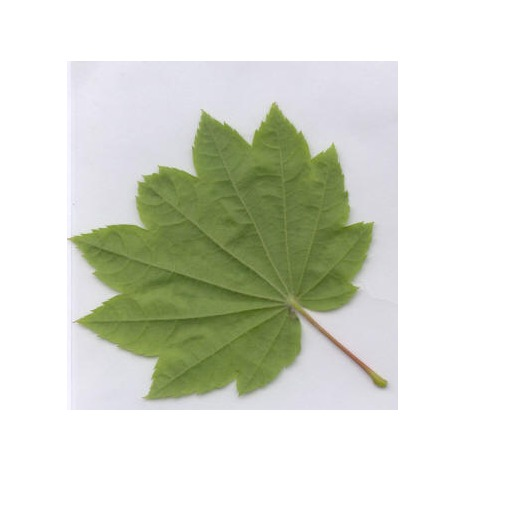
\includegraphics[width=\textwidth]{circinatum_sample.jpg}
\caption{Acer Circinatum\\Vine Maplel}
\end{subfigure}
\begin{subfigure}[b]{0.3\textwidth}
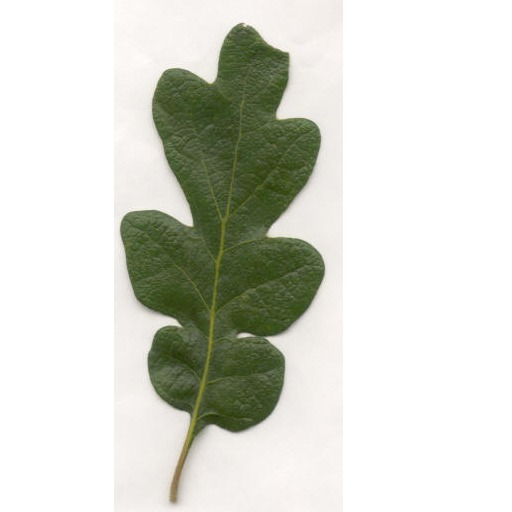
\includegraphics[width=\textwidth]{garryana_sample.jpg}
\caption{Quercus Garryana\\Oregon White Oak}
\end{subfigure}\\
\begin{subfigure}[b]{0.3\textwidth}
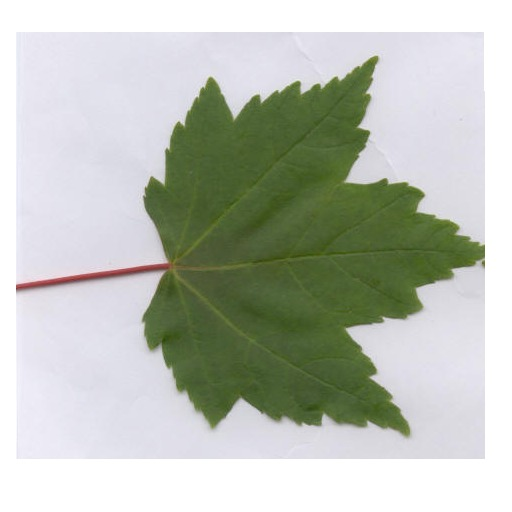
\includegraphics[width=\textwidth]{glabrum_sample.jpg}
\caption{Acer Glabrum\\Douglasii}
\end{subfigure}
\begin{subfigure}[b]{0.3\textwidth}
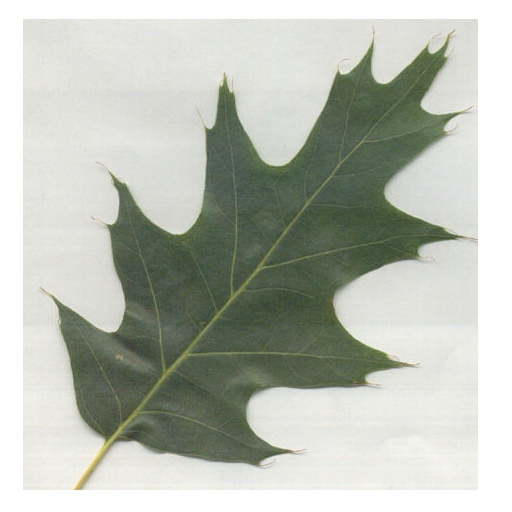
\includegraphics[width=\textwidth]{kelloggii_sample.jpg}
\caption{Quercus Kelloggii\\California Black Oak}
\end{subfigure}\\
\begin{subfigure}[b]{0.3\textwidth}
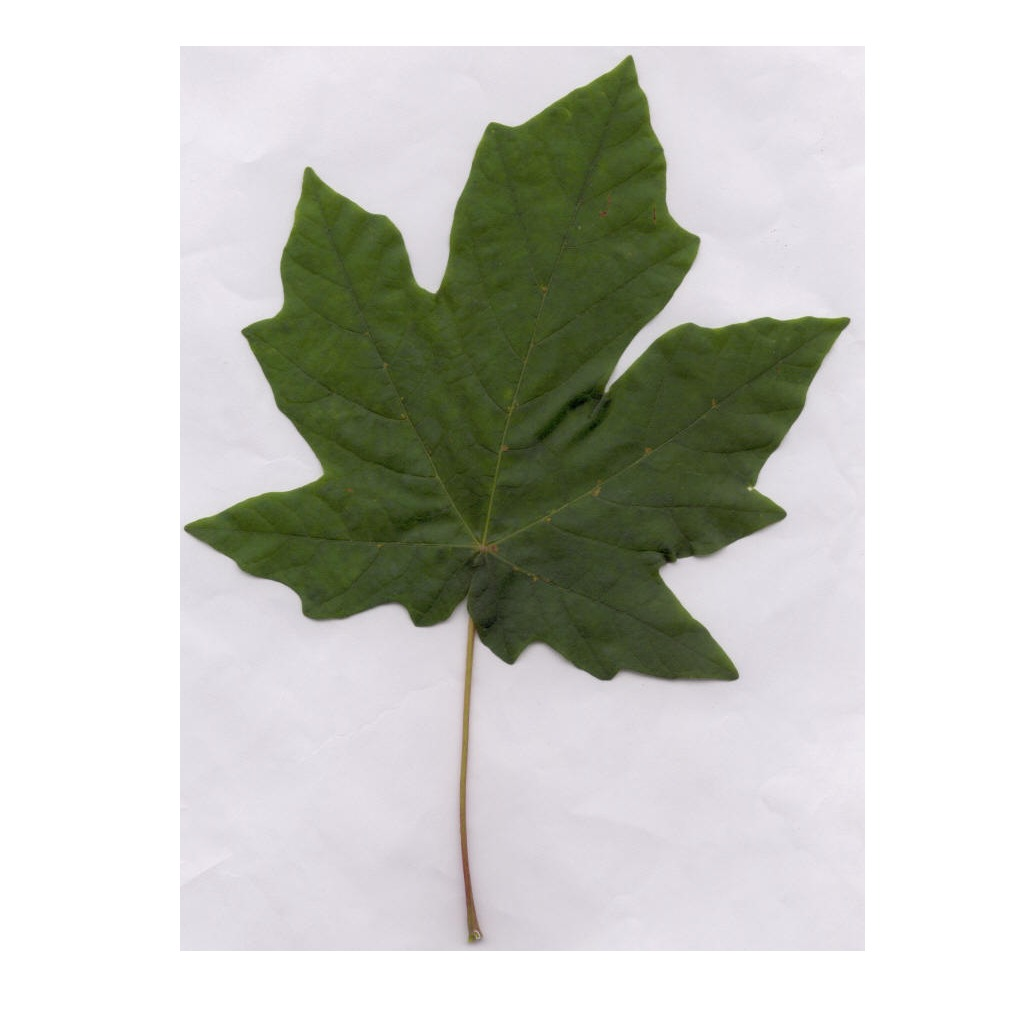
\includegraphics[width=\textwidth]{macrophyllum_sample.jpg}
\caption{Acer Macrophyllum\\Big Leaf Maple}
\end{subfigure}
\begin{subfigure}[b]{0.3\textwidth}
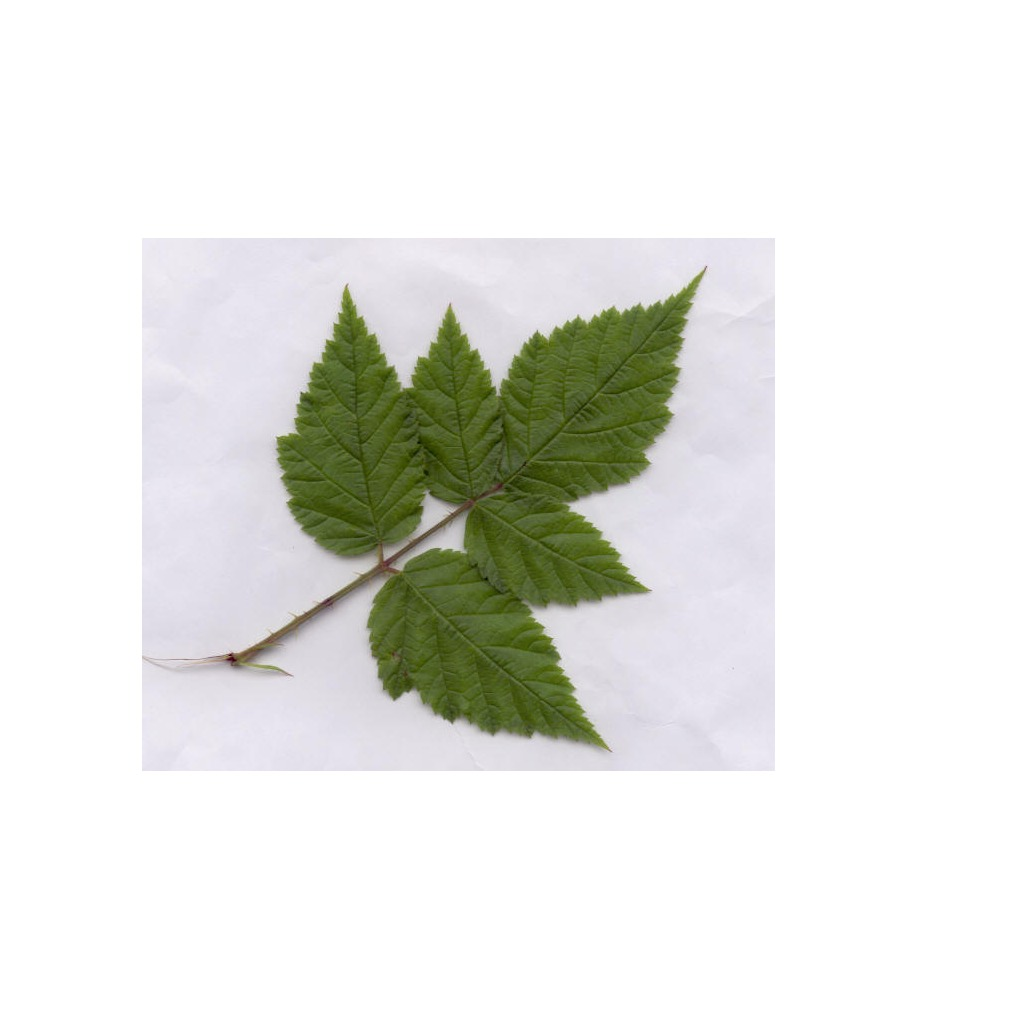
\includegraphics[width=\textwidth]{negundo_sample.jpg}
\caption{Acer Negundo\\Boxelder}
\end{subfigure}
\caption{Pictures of leaves}
\end{figure}

\subsection{Project Description}

\subparagraph{
For classification, I chose a random forest method, which is the ensemble learning method for classification, regression and other tasks that operates by constructing a multitude of decision trees. All images are analyzed by 6 descriptors, all of them are used to learn the algorithm and after that to recognise images from the test set. For all-purpose, I prepared 5 python files.\\\\
}

List of files :
\begin{itemize}
\item descriptors.py - contains all descriptors functions
\item summary.py - uses to save all results in files
\item separate\_images.py - copy files to "train\&test" directory and separate them to train and test sets
\item train\_test.py - the main file contains all train and test functions
\item cross\_validation.py - file contains function with cross-validation
\end{itemize}

\newpage

\section{Classification}

\paragraph{
In the section is described the process of classification leaves, using the descriptors and training and testing model.
}

\subsection{Feature Descriptors}

\subparagraph{
The subsection includes descriptions of all descriptors.
}

\subsubsection{Hu Moments}

Hu moments are used to calculate moments that are invariant to translation, scale, and rotation. The feature descriptor is in the first function in "descriptors.py". For clarify, an image moment is a certain particular weighted average (moment) of the image pixels' intensities or a function of such moments, usually chosen to have some attractive property or interpretation.

\begin{lstlisting}[language=Python]
# Hu Moments
def fd_hu_moments(image):
gray = cv2.cvtColor(image, cv2.COLOR_BGR2GRAY)
feature = cv2.HuMoments(cv2.moments(gray)).flatten()
return feature
\end{lstlisting}

This is a simple function. It takes as an input the only image, changes the image's colors to black and white and computes Hu Moments. In the end, it flattens the results to one array.

\subsubsection{Haralick Texture}

Texture defines the consistency of patterns and colors in an image. Haralick suggested the use of grey level co-occurrence matrices (GLCM). The basic idea of GLCM - it looks for pairs of adjacent pixel values that occur in an image and keeps recording it over the entire image. The Haralick Texture is computed in the second function in "descriptors.py".

\begin{lstlisting}[language=Python]
# Haralick Texture
def fd_haralick(image):
gray = cv2.cvtColor(image, cv2.COLOR_BGR2GRAY)
haralick = mahotas.features.haralick(gray).mean(axis=0)
return haralick
\end{lstlisting}

The function is simple, takes the only image as input, and return haralick descriptor. Firstly it changes the colors of the image to black and white. After that using mahotas library function computes the feature descriptor.

\subsubsection{Color Histogram}

In image processing and photography, a color histogram is a representation of the distribution of colors in an image. For digital images, a color histogram represents the number of pixels that have colors in each of a fixed list of color ranges, that span the image's color space, the set of all possible colors. The ranges convert to the vector is the result of the third feature descriptor in "descriptors.py".

\begin{lstlisting}[language=Python]
# Color Histogram
def fd_histogram(image):
hist = cv2.calcHist([image], [0, 1, 2], None, [8, 8, 8], [0, 256, 0, 256, 0, 256])
cv2.normalize(hist, hist)
return hist.flatten()
\end{lstlisting}

The function is even easier than the previous two. The descriptor for computation needs the only image. Then even no changes of colours are required. Using the OpenCV library and the calcHist method the function compute the histogram. After that, the histogram is normalized and returned flattened.

\subsubsection{Histogram of Oriented Gradients}

The Histogram of Oriented Gradients descriptor technique counts occurrences of gradient orientation in localized portions of an image.
The feature descriptor is computed as the fourth one in descriptors.py".

\begin{lstlisting}[language=Python]
# Histogram of Oriented Gradients
def fd_histog(image):
gray = cv2.cvtColor(image, cv2.COLOR_BGR2GRAY)
h = feature.hog(gray, orientations=9, pixels_per_cell=(8, 8),
cells_per_block=(2, 2), transform_sqrt=True, block_norm="L1")
return h
\end{lstlisting}

As the rest descriptor functions, the one takes the only image as input also. Then changing the colors to black and white occurs. The feature library helps with the computing of the histogram of the oriented gradients. And the result of the hog method is returned.

\subsubsection{Local Binary Pattern}

In the whole project is only two local descriptors - the first one Local Binary Pattern, which computes a local representation of texture.
The input image is changed to the black-and-white photo, then using feature library and its method local\_binary\_pattern compute the descriptor.

\begin{lstlisting}[language=Python]
def fd_binary_pattern(image):
gray = cv2.cvtColor(image, cv2.COLOR_BGR2GRAY)
lbp = feature.local_binary_pattern(gray, 24, 8, method="uniform")
(hist, _) = np.histogram(lbp.ravel(),
bins=np.arange(0, 27),
range=(0, 26))
hist = hist.astype("float")
hist /= (hist.sum() + 1e-7)
return hist
\end{lstlisting}

\subsubsection{Oriented FAST and rotated BRIEF}

The second local descriptor is Oriented FAST and rotated BRIEF. For the one, the results were different for each kind of tree. To prevent the different length of the descriptor vector, after computing the descriptor the length is changed to 100. If the vector has less then 100 values the remaining is a sequence of zeros, in another case when vector has more than 100 values only the first hundred is taken as the result.

\begin{lstlisting}[language=Python]
# Oriented FAST and rotated BRIEF
def fd_orb(image):
orb = cv2.ORB_create(nfeatures=100)
keypoints = o.detect(image,None)
keypoints, descriptors = o.compute(image, keypoints)
descriptors=descriptors.flatten()
if len(descriptors)<100:
descriptors = np.zeros(100-len(descriptors),dtype=int)
else:
descriptors = np.array(descriptors[0:100])
return descriptors
\end{lstlisting}

\subsubsection{Unused}

I prepared Scale Invariant Feature Transform descriptor also but the method SIFT\_create() from cv2.xfeatures2d returned the communication "This algorithm is patented and is excluded in this configuration". So that I decided not to use the descriptor in the project.

\begin{lstlisting}[language=Python]
# SIFT
def fd_SIFT(image):
gray = cv2.cvtColor(image, cv2.COLOR_BGR2GRAY)
freakExtractor = cv2.xfeatures2d.FREAK_create()
keypoints,descriptors= freakExtractor.compute(gray,None)
return keypoints
\end{lstlisting}

After searching for information, I found the free version of SIFT algorithm but it does not return any features. The algorithm throws an error because the machine learning model cannot learn from an empty feature vector. So as in the upper case, I decided to not use the descriptor in the project.

\begin{lstlisting}[language=Python]
# SIFT v2
def fd_SIFT_v2(image):
gray= cv2.cvtColor(image,cv2.COLOR_BGR2GRAY)
sift = cv2.xfeatures2d.SIFT_create()
kp = sift.detect(gray,None)
image=cv2.drawKeypoints(gray,kp,image)
cv2.show('sift_keypoints.jpg',image)
return kp
\end{lstlisting}

\newpage

\subsection{Cross validation}

\subparagraph{Cross-validation is a process which predicts the ML model's accuracy.}

In the project is used 10-fold cross-validation which means that the data set is divided into 10 subsets. The algorithm predicts the result 10 times, every time 9 sets are used to train and one for tests. Each iteration other set is the test one, so for each set is once used for test and nine times for train. The average of the ten results is returned.

\begin{lstlisting}[language=Python]
print("10-fold cross validation")
class_names = ["circinatum", "garryana", "glabrum", "kelloggii", "macrophyllum","negundo"]
all_descriptors = []
labels = []
for label in class_names:
for jpgfile in glob.glob("isolated/"+label+"/*.jpg"):
image = cv2.imread(jpgfile)
image = cv2.resize(image, (512,512))
\end{lstlisting}

Every image in the data set is loaded and resize to the same dimensions.

\begin{lstlisting}[language=Python]
fv_hu_moments = fd_hu_moments(image)
fv_haralick   = fd_haralick(image)
fv_histogram  = fd_histogram(image)
fv_hog        = fd_histog(image)
fv_binpat     = fd_binary_pattern(image)
fv_orb        = fd_orb(image)
fv_SIFT       = fd_SIFT(image)
# save them in descriptors variable
 descriptors = np.hstack([fv_histogram , fv_haralick, fv_hu_moments , fv_hog , fv_binpat, fv_orb])
\end{lstlisting}

The stack of descriptors is saved in all\_descriptors list and kind of tree is saved in labels list.

\begin{lstlisting}[language=Python]
# save labels and feature as the vectors
labels.append(label)
all_descriptors.append(descriptors)
\end{lstlisting}

Then from the library "sklearn.model\_selection" take KFold function and prepare the algorithm for 10-fold cross-validation.
After that function creates the ML model - Random Forest Classifier. In the end, the function computes the cross-validation and print mean and standard deviation of the ten results fo the 10-fold algorithm.

\begin{lstlisting}[language=Python]
# # 10-fold cross validation
kfold = KFold(n_splits=10)
rf = RandomForestClassifier(n_estimators=100, random_state=9)
cv_results = cross_val_score(rf, train_data, train_labels, cv=kfold, scoring="accuracy")
msg = "%s: %f (%f)" % ('RF', cv_results.mean(), cv_results.std())
print(msg)
\end{lstlisting}

\newpage

\subsection{Division of data set}

\subparagraph{
For classification purposes, the data set has to be split into two parts. The first with 80\% of all images are used to train the method. The second with remaining 20\% is used for test of the method. \\\\
}

In "separete\_images.py" I prepared to function for split the data set.

\begin{lstlisting}[language=Python]
class_names = ["circinatum", "garryana", "glabrum", "kelloggii", "macrophyllum","negundo"]
directory = "train&test"

def separeteImages():
\end{lstlisting}

Firstly, the program creates new empty directories to store the images.

\begin{lstlisting}[language=Python]
# create new empty directories
if os.path.exists(directory):
shutil.rmtree(directory, ignore_errors=True)
os.makedirs(directory)
\end{lstlisting}

Next, for every kind of tree create test and train directories.

\begin{lstlisting}[language=Python]
# for every spiece
for image in class_names:
# prepare two directories
# one for train images
train_dir = directory+"/"+image
os.mkdir(train_dir)
train_dir += "/train"
os.mkdir(train_dir)
# one for test images
test_dir = directory+"/"+image+"/test"
os.mkdir(test_dir)
\end{lstlisting}

After that, the program start splitting all photos in the set

\begin{lstlisting}[language=Python]
# for every image in data set
i=0
for jpgfile in glob.glob("isolated/"+image+"/*.jpg"):
if(i%5==0):
shutil.copy(jpgfile, test_dir)
else:
shutil.copy(jpgfile, train_dir)
i+=1
\end{lstlisting}

Every image with index number equal modulo to 5 is saved in the test directory, and the rest are stored in train directory.
For comparison of the descriptors, I preformed the code only once at the start of the project. The fact provides that for all results algorithm always has the same input data.

\newpage

\subsection{Train and test}

\subparagraph{
The section covers the most important part of the project. Here is the description of the main algorithm which learn the ML model and after that tests the results. The algorithm is included in "train\_test.py" \\\\
}

At the start, the program reads all imagines in train directories from all species and resize all of them to common dimensions.

\begin{lstlisting}[language=Python]
all_descriptors = []
labels = []
# learning from the train directories
for label in class_names:
for file in glob.glob('train&test/'+(label)+'/train/*.jpg'):
# read the image and resize it to the common size
image = cv2.imread(file)
image = cv2.resize(image, (512,512))
\end{lstlisting}

For each image, all descriptors are computed and saved in all\_descriptors list, while the species names of the images are stored in labels list.

\begin{lstlisting}[language=Python]
# compute descriptors
fv_hu_moments = fd_hu_moments(image)
fv_haralick   = fd_haralick(image)
fv_histogram  = fd_histogram(image)
fv_hog        = fd_histog(image)
fv_binpat     = fd_binary_pattern(image)
fv_orb        = fd_orb(image)
# fv_SIFT       = fd_SIFT(image)  
# save them in descriptors variable
descriptors = np.hstack([fv_histogram, fv_haralick, fv_hu_moments, fv_hog, fv_binpat, fv_orb])
# save labels and feature as the vectors
labels.append(label)
all_descriptors.append(descriptors)
\end{lstlisting}

When the training set of data completed, the program creates the Random Forest Classifier and learns the ML model.

\begin{lstlisting}[language=Python]
# Random Forests Classifier
clf = RandomForestClassifier(n_estimators=100, random_state=9)
# learning the model
clf.fit(all_descriptors, labels)
\end{lstlisting}

When learning is done, the algorithm starts testing section by reads all images and resize them.

\begin{lstlisting}[language=Python]
for label in class_names:
for file in glob.glob('train&test/'+(label)+'/test/*.jpg'):
# read the image and resize it to the common size
image = cv2.imread(file)
image = cv2.resize(image, (512,512))
\end{lstlisting}

Once again program computes all descriptors but in the case for the testing images.

\begin{lstlisting}[language=Python]
        # compute descriptors
        fv_hu_moments = fd_hu_moments(image)
        fv_haralick   = fd_haralick(image)
        fv_histogram  = fd_histogram(image)
        fd_hog        = fd_histog(image)
        fd_binpat     = fd_binary_pattern(image)
        fv_orb        = fd_orb(image)
        # fv_SIFT       = fd_SIFT(image)
        # save them in descriptors variable
        descriptors = np.hstack([fv_histogram, fv_haralick, fv_hu_moments, fv_hog, fv_binpat, fv_orb])
\end{lstlisting}

Next step is the prediction and checking the results. Name of the kind of tree is printed out with the predicted name. User can easily and in real-time check the results.

\begin{lstlisting}[language=Python]
prediction = clf.predict(descriptors.reshape(1,-1))[0]
print(label,prediction)
results.append((label,prediction))
\end{lstlisting}

All of the results are stored in the results list. The reason for that is an optional function which can save the data to files and computes the mean.
The function "save\_and\_summary" is described in the next subsection.

\begin{lstlisting}[language=Python]
save_and_summary(results)
\end{lstlisting}

\newpage

\subsection{Summary}

\subparagraph{
For saving results for each image, each kind of tree and for all data set I prepared summary.py file. \\\\
}

At first, the program creates empty files in directory "test\&file". AllResults.txt file includes all results in form "kind of tree"
$\rightarrow$
"prediction", and Summary.txt file includes a summary for each class and whole data set.

\begin{lstlisting}[language=Python]
# function for save results and summary
def save_and_summary( results ):
# create files to save results
if not os.path.exists("./train&test"):
os.makedirs("./train&test")
AllResults = open("./train&test/AllResults.txt" , 'w')
Summary = open("./train&test/Summary.txt" , 'w')
\end{lstlisting}

\begin{center}
\begin{figure}[h!]
\centering
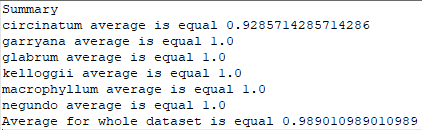
\includegraphics[width = 4in]{summary_sample.png}
\end{figure}
\end{center}

\begin{center}
\begin{figure}[h!]
\centering
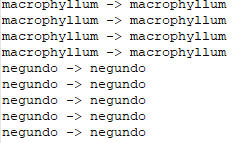
\includegraphics[width =3in]{allresults_sample.png}
\end{figure}
\end{center}

Variable "results" is a list of tuples with the correct answer at the \nth{1} position and prediction of the model at the \nth{2} position in each tuple.

\begin{lstlisting}[language=Python]
# from train&test.py
results.append((label,prediction))
\end{lstlisting}

Then create two dictionaries and save the results to AllResults.txt. In the same loop compute the number of correct predictions.

\begin{lstlisting}[language=Python]
# create 2 dictionaries for computing correct preditions
num = dict()
den = dict()
for name in class_names:
num[name] = 0
den[name] = 0
for result in results:
# write all preditions to AllResults file
AllResults.write(' -> '.join(result)+'\n')
# compute correctness for each spiecie
den[result[0]] += 1
if result[0] == result[1]:
num[result[0]] += 1
\end{lstlisting}

In the next step, the program starts summary. Firstly, compute the result for each kind of tree.

\begin{lstlisting}[language=Python]
n = 0
d = 0
# Summary
Summary.write("Summary\n")
for name in class_names:
# write results for each class
if den[name] != 0:
line = name+" average is equal "+ str(num[name]/den[name])
Summary.write(line+"\n")
print(line)
n += num[name]
d += den[name]
\end{lstlisting}

Then it computes mean for all data set.

\begin{lstlisting}[language=Python]
if d != 0:
# write result for whole data set
line = "Average for whole dataset is equal "+ str(n/d)
Summary.write(line+"\n")
print(line)
\end{lstlisting}

At the end close the files.

\newpage

\section{Results}

\subsection{10-fold cross validataion}

\subparagraph{
For better results I prepared 10-fold cross validataion for whole set of data.\\\\
}

The 10-fold algorithm divides the set into 10 parts and checks the results of machine learning for each set as the test one and rest as the training. Then mean of all 10 outputs it the finite result. The image below shows the results for all descriptors.

\begin{figure}[h!]
\centering
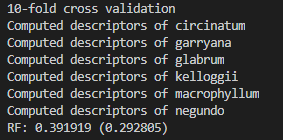
\includegraphics[width=3in]{Cross_1.png}
\end{figure}

The mean is only 40\%. However, for the 3 descriptors (Hu moments, Haralick Texture, Color Histogram) the cross-validation result has the maximum mean which is equal to 89\%.


\begin{figure}[h!]
\centering
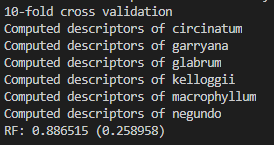
\includegraphics[width=3in]{Cross_for3.png}
\end{figure}

The most interesting fact is that if I had used only Color Histogram descriptor the results were close to the highest result.

\begin{figure}[h!]
\centering
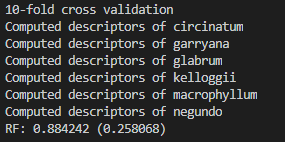
\includegraphics[width=3in]{Cross_histogram.png}
\end{figure}

So after adding 3 global and 2 local descriptors the result increases by only 0,2\%. The 5 remaining descriptors have result between 40\% and 70\%. The results are around 90\% of accuracy as the mean of 10-fold cross-validation.

\subsection{80\% training / 20\% testing}

\subparagraph{
In the project description stayed the statement that the whole data set should be divided into two parts. First with 80\% of the images as the training and rest 20\% as the test set. Using "separeteImages()" function which is described in the 2.3 section I divide the data and perform the test.\\\\
}

For the results, I prepared "save\_and\_summary( results )" function which is described in the 2.5 section. All the results are saved as text files. Moreover, each species has the mean results and each prediction is saved also. In the report, I show only the summary of the few sets of descriptors. Firstly the result for all descriptors.

\begin{figure}[h!]
\centering
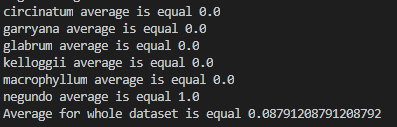
\includegraphics[width=3in]{results_1.png}
\end{figure}

The result is low - only 9\%. For the negundo kind, the result is equal to 100\% but this is the only class without 0\% as a result. However below is shown the image with the result using only 3 descriptors (Hu moments, Haralick Texture, Color Histogram).

\begin{figure}[h!]
\centering
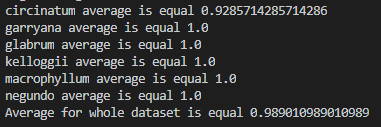
\includegraphics[width=3in]{results_3.png}
\end{figure}
For the 3 descriptors, the results are much better - around 99\%. And only for the circinatum kind of tree the results are not 100\% correct. And one more result of the comparison is presented below.

\begin{figure}[h!]
\centering
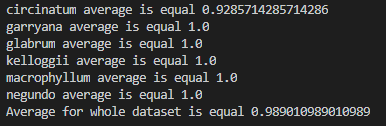
\includegraphics[width=3in]{results_histo.png}
\end{figure}

The results look like 2nd time the same image but this one is different - only Color Histogram was used to obtain the results. So in the case, the 5 descriptors (3 globals and 2 locals) do not affect the best result. The machine learning model correctly interprets the same number of images using only Color Histogram, the same number using the 3 descriptors and obtain better result then all set of descriptors. The 10-fold cross-validation shows the small difference but for the 80\% training / 20\% testing the results are the same.

\section{Source Code}

\subsection{descriptors.py}
\lstinputlisting[language=Python]{../descriptors.py}

\subsection{summary.py}
\lstinputlisting[language=Python]{../summary.py}

\subsection{separate\_images.py}
\lstinputlisting[language=Python]{../separate_images.py}

\subsection{train\_test.py}
\lstinputlisting[language=Python]{../train_test.py}

\subsection{cross\_validation.py}
\lstinputlisting[language=Python]{../cross_validation.py}

\newpage

\section{References}

\begin{enumerate}
\item \url{https://en.wikipedia.org/wiki/Random\_forest}
\item \url{https://gogul.dev/software/image-classification-python}
\item \url{https://www.learnopencv.com/histogram-of-oriented-gradients/}
\item \url{https://opencv-python-tutroals.readthedocs.io/en/latest/py_tutorials/py_feature2d/py_orb/py_orb.html}
\item \url{https://en.wikipedia.org/wiki/Image_moment}
\item \url{http://wiki.awf.forst.uni-goettingen.de/wiki/index.php/Haralick_Texture}
\item \url{https://software.intel.com/en-us/ipp-dev-reference-histogram-of-oriented-\\gradients-hog-descriptor}
\item \url{https://en.wikipedia.org/wiki/Color_histogram}
\item \url{https://software.intel.com/en-us/ipp-dev-reference-histogram-of-oriented-\\gradients-hog-descriptor}
\item \url{https://www.pyimagesearch.com/2015/12/07/local-binary-patterns-with-python-\\opencv/}

\end{enumerate}

\end{document}